\documentclass[kdmile,a4paper]{kdmile}

\usepackage[utf8]{inputenc}
\usepackage[T1]{fontenc}
\usepackage[brazil]{babel}
\usepackage{amsmath}
\usepackage{amssymb}
\usepackage{booktabs}
\usepackage{array}
\usepackage{graphicx,url}

\newtheorem{theorem}{Theorem}[section]
\newtheorem{conjecture}[theorem]{Conjecture}
\newtheorem{corollary}[theorem]{Corollary}
\newtheorem{proposition}[theorem]{Proposition}
\newtheorem{lemma}[theorem]{Lemma}
\newdef{definition}[theorem]{Definition}
\newdef{remark}[theorem]{Remark}

\markboth{J. T. A. Júnior and C. O. Caminha Neto}
{Specialized Detector or Vision-Language Model?}
\title{Specialized Detector or Vision-Language Model? Evaluating YOLOv11m and Gemma 3 27B-IT for Urban Waste Monitoring}

\author{Jaime Teixeira de Araújo Júnior\inst{1}, Carlos de Oliveira Caminha Neto\inst{1}}

\institute{Universidade Federal do Ceará -- Fortaleza -- CE -- Brasil\\
  \email{jaimejrs@alu.ufc.br, carlos.o.c.neto@gmail.com}
}

\begin{abstract}
Urban waste monitoring on public roads is a relevant challenge for municipal management because it requires large-scale inspection under limited operational resources. This study evaluates two distinct artificial intelligence strategies for identifying visible waste in real images of Brazilian streets: YOLOv11m, fine-tuned as a specialized object detector, and Gemma 3 27B-IT, employed as a zero-shot vision-language model. YOLOv11m was trained with 6,736 images, including 15.6\% background samples, while both models were evaluated on an external and balanced test set containing 560 Brazilian street images. Predictive performance, error profiles, statistical significance, latency, and throughput were analyzed. Gemma 3 27B-IT achieved higher accuracy, recall, specificity, and F1-score, obtaining an F1-score of 0.9238 against 0.7040 for YOLOv11m. The difference was statistically significant according to McNemar's test. Conversely, under the HTTP service flow evaluated here, YOLOv11m processed approximately 119 images per second and presented an average latency 141.9 times lower than the vision-language model. The findings reveal a clear accuracy--latency trade-off: Gemma is more suitable for targeted analyses that prioritize predictive performance, whereas YOLO is more appropriate for large-scale screening, real-time processing, and applications requiring explicit visual localization. The results also indicate potential for hybrid systems combining fast detection and multimodal confirmation.
\end{abstract}

\begin{CCSXML}
<ccs2012>
<concept>
<concept_id>10010147.10010257.10010258.10010259</concept_id>
<concept_desc>Computing methodologies~Object detection</concept_desc>
<concept_significance>500</concept_significance>
</concept>
<concept>
<concept_id>10010147.10010257.10010282</concept_id>
<concept_desc>Computing methodologies~Computer vision</concept_desc>
<concept_significance>500</concept_significance>
</concept>
<concept>
<concept_id>10010405.10010469.10010474</concept_id>
<concept_desc>Applied computing~Environmental sciences</concept_desc>
<concept_significance>300</concept_significance>
</concept>
</ccs2012>
\end{CCSXML}
\ccsdesc[500]{Computing methodologies~Object detection}
\ccsdesc[500]{Computing methodologies~Computer vision}
\ccsdesc[300]{Applied computing~Environmental sciences}

\keywords{object detection, public administration, urban waste monitoring, vision-language models, YOLOv11m}

\begin{document}

\begin{bottomstuff}
\end{bottomstuff}

\maketitle

\section{Introdução}
\label{sec:introducao}

A gestão de resíduos sólidos urbanos envolve impactos ambientais, sanitários, financeiros e operacionais. No Brasil, a Política Nacional de Resíduos Sólidos atribui aos municípios papel central na organização da coleta e destinação dos resíduos \cite{Brasil2010}, cujos custos dependem diretamente da estrutura operacional adotada \cite{Rodrigues2016}.

A produção de informações territorializadas sobre descarte irregular pode apoiar a priorização de áreas, o planejamento de rotas e a fiscalização. Entretanto, a inspeção manual de grandes volumes de imagens demanda tempo e recursos humanos. Técnicas de visão computacional oferecem a possibilidade de transformar registros visuais de ruas em alertas administrativos, mas sua utilidade depende não apenas da acurácia, como também da velocidade, da ocorrência de falsos alarmes, da rastreabilidade e da infraestrutura necessária para operação.

Detectores de objetos da família YOLO são orientados à localização rápida de instâncias visuais e retornam caixas delimitadoras que facilitam a auditoria das predições \cite{Redmon2016,Terven2023}. Modelos visão-linguagem, por sua vez, associam imagens e instruções textuais, podendo executar tarefas em regime \emph{zero-shot}, sem ajuste específico no conjunto-alvo \cite{Radford2021,Zhang2024}. Essa flexibilidade reduz o esforço inicial de treinamento, mas pode exigir modelos maiores e maior custo de inferência.

Estudos anteriores aplicaram redes profundas à detecção de resíduos em ambientes urbanos e naturais \cite{Cordova2022,Majchrowska2022}. Também surgiram avaliações de modelos visão-linguagem para classificação de resíduos \cite{Funk2025,Malla2026}. Contudo, permanece limitada a evidência sobre a comparação direta, no mesmo conjunto de imagens brasileiras, entre um detector especializado e um grande modelo visão-linguagem, considerando simultaneamente desempenho preditivo, significância estatística, latência e implicações administrativas.

Este trabalho investiga as seguintes perguntas de pesquisa:
\begin{itemize}
    \setlength{\itemsep}{0pt}
    \setlength{\parsep}{0pt}
    \setlength{\topsep}{2pt}
    \item \textbf{RQ1:} Como se comparam, em desempenho preditivo, um detector especializado com \emph{fine-tuning} e um VLM generalista em \emph{zero-shot} em imagens reais de vias públicas brasileiras?
    \item \textbf{RQ2:} Qual é o trade-off entre desempenho preditivo, eficiência computacional e adequação aos diferentes cenários de monitoramento urbano?
\end{itemize}

As principais contribuições são: uma avaliação controlada em 560 imagens brasileiras externas ao treinamento; a comparação entre um detector ajustado por \emph{fine-tuning} e um modelo visão-linguagem em regime \emph{zero-shot}; uma análise estatística pareada das predições; e a caracterização dos cenários em que cada paradigma apresenta maior viabilidade operacional.

\section{Trabalhos Relacionados}
\label{sec:trabalhos-relacionados}

\subsection{Detecção automatizada de resíduos}
\label{sec:deteccao-residuos}

A detecção de objetos busca identificar e localizar instâncias por meio de caixas delimitadoras. A família YOLO consolidou essa tarefa em uma etapa única de regressão, favorecendo aplicações de baixa latência e alto volume \cite{Redmon2016,Terven2023,Khanam2024}.

No domínio dos resíduos, o TACO reúne imagens reais com lixo deformado, fragmentado, transparente ou parcialmente oculto \cite{Proenca2020}. Estudos anteriores demonstram a viabilidade da detecção automatizada, mas também reportam dificuldades com objetos pequenos, oclusão, iluminação e deslocamento de domínio \cite{Majchrowska2022,Cordova2022}. Assim, detectores treinados em bases internacionais podem exigir adaptação para ruas brasileiras.

\subsection{Modelos visão-linguagem}
\label{sec:modelos-visao-linguagem}

Modelos visão-linguagem aprendem relações entre representações visuais e linguagem natural. A supervisão multimodal possibilita reconhecimento orientado por descrições textuais e execução de tarefas sem exemplos específicos do domínio-alvo \cite{Radford2021,Li2023}.

O Gemma 3 é uma família multimodal capaz de receber imagens e texto e produzir respostas orientadas por instruções \cite{GemmaTeam2025}. Embora modelos desse tipo ofereçam flexibilidade, pesquisas apontam desafios de estabilidade, alinhamento, \emph{grounding} visual, custo computacional e alucinações \cite{Li2025}. Estudos recentes avaliaram VLMs na classificação de resíduos em regime \emph{few-shot} e destilação para classificação eficiente \cite{Funk2025,Malla2026}. Diferentemente deles, este estudo avalia descarte em vias públicas brasileiras \emph{in-the-wild}, não triagem em instalações de recuperação de materiais ou classificação \emph{few-shot}, comparando diretamente um VLM generalista e um detector especializado sob métricas operacionais.

\section{Metodologia}
\label{sec:metodologia}

\subsection{Tarefa e dados}
\label{sec:tarefa-dados}

A unidade de análise foi a imagem. Cada amostra foi classificada como \textbf{com resíduo visível} ou \textbf{sem resíduo visível}, avaliando uma tarefa inicial de triagem binária. O treinamento do YOLOv11m utilizou imagens positivas das bases TACO e Trash Detection (agregadas na classe ``lixo'') e negativas da base Sidewalk Segmentation. Os conjuntos resultantes são detalhados na Tabela~\ref{tab:conjuntos}.

\begin{table}[htbp]
\centering
\footnotesize
\caption{Composição dos conjuntos experimentais}
\label{tab:conjuntos}
\begin{tabular}{lccc}
\toprule
\textbf{Conjunto} & \textbf{Total de Imagens} & \textbf{Positivas (com lixo)} & \textbf{Negativas (sem lixo)} \\
\midrule
Treinamento & 6.736 & 5.685 & 1.051 \\
Validação & 1.286 & 1.101 & 185 \\
Teste brasileiro & 560 & 280 & 280 \\
\bottomrule
\end{tabular}
\end{table}

As imagens do teste foram obtidas de registros reais de vias públicas brasileiras (plataformas urbanas, fotos próprias e projetos locais), mantidas separadas do treino. O \emph{ground truth} classificou como resíduos sacos, embalagens, garrafas, papelão e plásticos, enquanto lixeiras fechadas, vegetação e objetos utilitários foram classificados como não resíduos.

A integridade das divisões foi garantida via deduplicação perceptual com \emph{pHash} (distância máxima de 5), removendo 1.661 duplicatas das 10.211 imagens brutas, sem correspondências entre treino e teste. Rostos e placas foram anonimizados ou descartados.

\subsection{Modelos e configurações}
\label{sec:modelos-configuracoes}

O experimento comparou duas estratégias representativas de decisões reais de adoção: treinar um modelo especializado ou empregar um modelo generalista sem treinamento adicional. As configurações específicas são apresentadas na Tabela~\ref{tab:configuracao}.

\begin{table}[htbp]
\centering
\footnotesize
\caption{Configuração dos modelos experimentais}
\label{tab:configuracao}
\begin{tabular}{lp{4.2cm}p{5.2cm}}
\toprule
\textbf{Configuração} & \textbf{YOLOv11m} & \textbf{Gemma 3 27B-IT} \\
\midrule
Regime & \emph{Fine-tuning} supervisionado & \emph{Zero-shot} \\
Saída principal & Caixas e confiança & Classe binária em JSON \\
Pesos/configuração & \emph{yolo11m.pt} & Quantização Q5\_K\_M \\
Épocas & 100 & Não aplicável \\
Resolução & 640 $\times$ 640 & Imagem original processada pelo servidor \\
\emph{Batch size} & 12 & Inferência individual \\
Otimizador & AdamW & Não aplicável \\
Taxa de aprendizado inicial & 0,001 & Não aplicável \\
\emph{Early stopping} & Paciência 20 & Não aplicável \\
\emph{Augmentation} & \emph{mosaic=1.0}, \emph{fliplr=0.5} & Não aplicável \\
Limiar principal & 0,25 & Resposta binária \\
Temperatura & Não aplicável & 0 \\
\emph{Seed} & Configuração do experimento & 42 \\
\bottomrule
\end{tabular}
\end{table}

O melhor \emph{checkpoint} do YOLO foi selecionado via validação (limiar de detecção $\ge 0,25$). O Gemma 3 27B-IT (quantização Q5\_K\_M) foi executado no LM Studio com temperatura zero, respondendo via JSON estruturado. 

Para a inferência do Gemma 3, o prompt em inglês definiu a tarefa: \emph{``You are a public street monitoring analyst. Your task is to answer one single question: IS THERE TRASH or discarded WASTE in this street image? Consider as trash: garbage bags, bottles, cans, cardboard, packaging, plastics, glass, or any discarded waste on a public street or sidewalk. Do NOT consider as trash: closed trash bins/containers in normal use, vehicles, people, vegetation, street furniture in good condition, or normal pavement. Respond STRICTLY in valid JSON, with no markdown and no text outside the JSON. Use exactly these field names: \{"tem\_lixo": true, "descricao\_breve": "...", "confianca": 0.0\}. If there is no visible trash, return tem\_lixo: false.''}. 

Para lidar com saídas fora do formato esperado, implementou-se um parser robusto que isola a estrutura JSON por captura de chaves (\emph{brackets matching}) e valida o resultado com \emph{jsonschema}. Caso o parsing falhasse por completo ou ocorresse timeout na requisição HTTP, a imagem seria conservadoramente rotulada como classe negativa (sem resíduos). No experimento de teste, contudo, todas as 560 inferências foram analisadas e estruturadas com sucesso pelo parser.

\subsection{Avaliação}
\label{sec:avaliacao}

Foram calculadas acurácia, precisão, sensibilidade, especificidade, F1-score, taxa de falsos positivos, kappa de Cohen, coeficiente de correlação de Matthews e matrizes de confusão. O mAP não foi empregado como métrica comparativa principal porque o Gemma produziu uma classificação por imagem, sem caixas delimitadoras. A comparação foi, portanto, realizada em nível binário de imagem para ambos os modelos.

Intervalos de confiança de 95\% foram estimados pelo método de Wilson e as discordâncias avaliadas pelo teste de McNemar. A latência e o \emph{throughput} foram medidos em uma GPU RTX 5090. No YOLO, o tempo incluiu a leitura local e inferência; no Gemma, o tempo decorrido entre a requisição HTTP e a resposta.

\section{Resultados e Discussão}
\label{sec:resultados}

\subsection{Desempenho preditivo}
\label{sec:desempenho-preditivo}

A Tabela~\ref{tab:desempenho} apresenta as métricas obtidas no conjunto de 560 imagens.

\begin{table}[htbp]
\centering
\footnotesize
\caption{Desempenho preditivo dos modelos}
\label{tab:desempenho}
\begin{tabular}{lccc}
\toprule
\textbf{Métrica} & \textbf{YOLOv11m} & \textbf{Gemma 3 27B-IT} & \textbf{Diferença} \\
\midrule
Acurácia & 0,7071 & 0,9179 & +0,2108 \\
Precisão & 0,7117 & 0,8611 & +0,1494 \\
Sensibilidade & 0,6964 & 0,9964 & +0,3000 \\
Especificidade & 0,7179 & 0,8393 & +0,1214 \\
F1-score & 0,7040 & 0,9238 & +0,2198 \\
Taxa de falsos positivos & 0,2821 & 0,1607 & $-0,1214$ \\
MCC & 0,4140 & 0,8460 & +0,4320 \\
Kappa de Cohen & 0,4140 & 0,8360 & +0,4220 \\
\bottomrule
\end{tabular}
\end{table}

O Gemma apresentou vantagem em todas as métricas preditivas. A diferença mais expressiva ocorreu na sensibilidade: o modelo identificou 279 das 280 imagens positivas (apenas 1 falso negativo), enquanto o YOLO identificou 195 (85 falsos negativos). A matriz de confusão também mostra que o modelo visão-linguagem apresentou maior capacidade de rejeitar cenas negativas (Tabela~\ref{tab:confusao}). Em uma aplicação pública, falsos negativos representam descarte não identificado, enquanto falsos positivos geram custos desnecessários de deslocamento de equipes e revisões manuais.

Os intervalos de confiança de 95\% da acurácia foram 0,668--0,743 para YOLO e 0,892--0,938 para Gemma. O teste de McNemar confirmou significância estatística ($\chi^2 = 74,40$, $p \approx 6,4 \times 10^{-18}$), com o Gemma acertando 151 imagens exclusivamente contra 33 do YOLO, respondendo à \textbf{RQ1}.

\begin{table}[htbp]
\centering
\footnotesize
\caption{Matrizes de confusão dos modelos experimentais}
\label{tab:confusao}
\begin{tabular}{lcccc}
\toprule
\textbf{Modelo} & \textbf{VP} & \textbf{VN} & \textbf{FP} & \textbf{FN} \\
\midrule
YOLOv11m & 195 & 201 & 79 & 85 \\
Gemma 3 27B-IT & 279 & 235 & 45 & 1 \\
\bottomrule
\end{tabular}
\par\smallskip\raggedright
\scriptsize Nota: VP = Verdadeiros Positivos; VN = Verdadeiros Negativos; FP = Falsos Positivos; FN = Falsos Negativos.
\end{table}

\subsection{Sensibilidade ao limiar do YOLO}
\label{sec:sensibilidade-limiar}

O limiar de confiança altera o equilíbrio entre sensibilidade e falsos positivos. A Tabela~\ref{tab:limiar_yolo} apresenta os quatro pontos de operação avaliados para o YOLOv11m.

\begin{table}[htbp]
\centering
\footnotesize
\caption{Sensibilidade ao limiar de confiança do YOLOv11m}
\label{tab:limiar_yolo}
\begin{tabular}{lcccccc}
\toprule
\textbf{Limiar} & \textbf{Acurácia} & \textbf{Precisão} & \textbf{Sensibilidade} & \textbf{Especificidade} & \textbf{F1-score} & \textbf{FPR} \\
\midrule
0,25 & 0,7071 & 0,7117 & 0,6964 & 0,7179 & 0,7040 & 0,2821 \\
0,35 & 0,7268 & 0,7617 & 0,6464 & 0,8071 & 0,6967 & 0,1929 \\
0,50 & 0,7054 & 0,8182 & 0,5464 & 0,8643 & 0,6548 & 0,1357 \\
0,65 & 0,6661 & 0,8737 & 0,4286 & 0,9036 & 0,5746 & 0,0964 \\
\bottomrule
\end{tabular}
\par\smallskip\raggedright
\scriptsize Nota: FPR = Taxa de Falsos Positivos (\emph{False Positive Rate}).
\end{table}

O aumento do limiar reduz falsos positivos, mas eleva substancialmente as omissões. Em 0,65, a especificidade supera 0,90, porém a sensibilidade cai para 0,4286. Assim, o ponto de operação não deve ser escolhido apenas pela maior acurácia, mas pelo custo relativo dos erros. Para uma triagem ampla, limiares menores podem ser aceitáveis quando alertas passam por validação posterior. Para acionamento automático de equipes, um limiar maior pode reduzir custos, mas aumentaria a quantidade de ocorrências não identificadas.

\subsection{Eficiência computacional}
\label{sec:eficiencia-computacional}

A vantagem preditiva do Gemma foi acompanhada por custo computacional significativamente maior, conforme detalhado na Tabela~\ref{tab:eficiencia}.

\begin{table}[htbp]
\centering
\footnotesize
\caption{Eficiência computacional dos modelos}
\label{tab:eficiencia}
\begin{tabular}{lcc}
\toprule
\textbf{Métrica} & \textbf{YOLOv11m} & \textbf{Gemma 3 27B-IT} \\
\midrule
Latência média & 8,4 ms & 1.191,9 ms \\
Mediana & 8,4 ms & 1.172,2 ms \\
Percentil 95 & 9,3 ms & 1.346,9 ms \\
Throughput & 119 imagens/s & 0,839 imagem/s \\
\bottomrule
\end{tabular}
\end{table}

A latência média do Gemma foi aproximadamente 141,9 vezes maior. O YOLO, portanto, apresenta clara vantagem quando há transmissão contínua, alto volume ou necessidade de resposta próxima ao tempo real. A comparação de latência deve ser interpretada como uma avaliação dos fluxos implementados, não como uma comparação isolada do tempo interno das arquiteturas. O Gemma foi acessado por interface HTTP e servidor intermediário, enquanto o YOLO foi executado diretamente no ambiente local. Ainda assim, a diferença superior a duas ordens de magnitude é operacionalmente relevante. Em resposta à \textbf{RQ2}: o Gemma oferece maior qualidade preditiva, enquanto o YOLO oferece velocidade, menor custo por imagem e localização explícita dos objetos. A Figura~\ref{fig:tradeoff-f1-latencia} sintetiza esse compromisso.

\begin{figure}[htbp]
\centering
\IfFileExists{outputs/figures/fig_tradeoff_f1_latencia.png}{%
  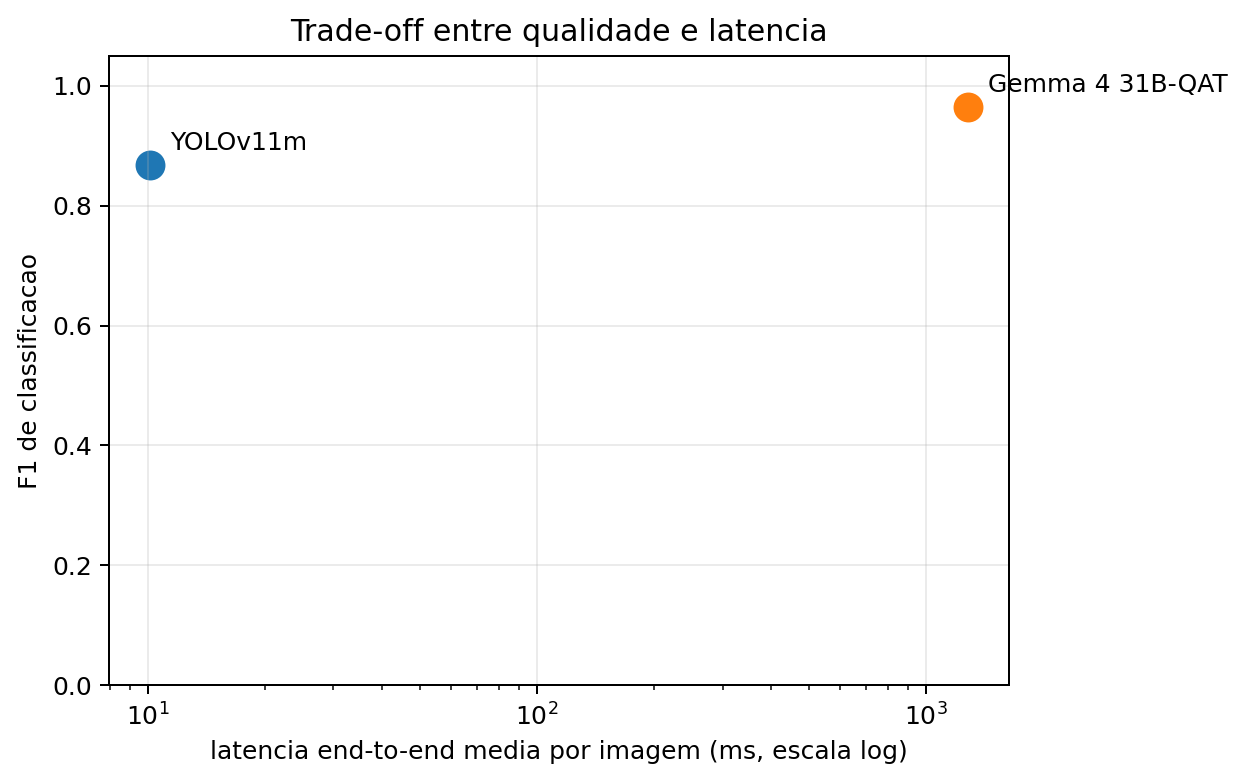
\includegraphics[width=0.48\linewidth]{outputs/figures/fig_tradeoff_f1_latencia.png}%
}{%
  \fbox{\parbox{0.46\linewidth}{\centering Figura de trade-off não encontrada. Execute o notebook para gerar o PNG.}}%
}
\caption{Trade-off entre F1-score e latência média end-to-end. Pontos mais próximos do canto superior esquerdo indicam maior desempenho com menor custo temporal.}
\label{fig:tradeoff-f1-latencia}
\end{figure}

\subsection{Análise dos erros e complementaridade}
\label{sec:analise-erros}

Os modelos acertaram conjuntamente 363 imagens (64,8\% do teste). Apenas o Gemma acertou 151 imagens; apenas o YOLO acertou 33; e ambos erraram 13. Nos falsos negativos do YOLO foram observados resíduos amassados, molhados, dispersos ou misturados ao pavimento, além de variações de iluminação, perspectiva e enquadramento. Algumas omissões ocorreram mesmo quando os resíduos eram visualmente relevantes, sugerindo possível deslocamento de domínio. Por outro lado, o Gemma apresentou somente um falso negativo, mas produziu 45 falsos positivos. Sua elevada sensibilidade indica capacidade de interpretar sinais contextuais da cena, mas essa mesma interpretação pode resultar em sobre-sinalização de objetos associados a descarte, mesmo na ausência de resíduos. Essas discordâncias sugerem complementaridade parcial: um sistema híbrido poderia empregar o YOLO na primeira etapa, processando rapidamente grandes volumes, e encaminhar imagens de baixa confiança ao Gemma. Tal estratégia deve ser avaliada em novos experimentos.

\subsection{Implicações para a gestão pública}
\label{sec:implicacoes-gestao}

Os resultados sugerem três usos principais: em monitoramento contínuo ou de alto volume, o YOLOv11m é preferível pela baixa latência, alto \emph{throughput} e disponibilidade de caixas delimitadoras; em auditorias ou análises pontuais, o Gemma 3 27B-IT é mais indicado quando a qualidade preditiva prevalece sobre o tempo de resposta; e, em triagens seguidas de confirmação, uma arquitetura híbrida pode combinar a velocidade do detector com a sensibilidade do VLM em casos selecionados. Em todos os cenários, a adoção deve incluir revisão humana, registro de alertas, auditoria de decisões, monitoramento de desempenho e reavaliação periódica frente a mudanças no ambiente urbano \cite{Zuiderwijk2021,Misic2025}.

\section{Ameaças à Validade}
\label{sec:ameacas-validade}

As principais ameaças à validade são:
\begin{itemize}
    \setlength{\itemsep}{0pt}
    \setlength{\parsep}{0pt}
    \setlength{\topsep}{2pt}
    \item teste balanceado artificialmente (50\% positivo), diferente da prevalência real em vias públicas;
    \item anotação por um único pesquisador, com possíveis ambiguidades de julgamento;
    \item assimetria experimental entre YOLO com \emph{fine-tuning} e Gemma em \emph{zero-shot};
    \item possível \emph{domain shift} entre TACO/Trash Detection e imagens urbanas brasileiras;
    \item latência do Gemma medida via LM Studio em Q5\_K\_M, sem avaliar concorrência, energia ou custos em produção.
\end{itemize}

\section{Conclusão}
\label{sec:conclusao}

Este trabalho comparou YOLOv11m e Gemma 3 27B-IT no monitoramento binário de resíduos em 560 imagens reais de vias públicas brasileiras. Em resposta à \textbf{RQ1}, a estratégia zero-shot com Gemma apresentou melhor desempenho preditivo no conjunto avaliado: F1-score de 0,9238 contra 0,7040 do YOLO, com superioridade estatisticamente significativa. Essa leitura depende do desenho experimental, pois o YOLO foi ajustado com bases públicas majoritariamente externas ao domínio das ruas brasileiras, sujeitas a \emph{domain shift}. Em resposta à \textbf{RQ2}, o YOLO apresentou vantagem expressiva em eficiência: 8,4 ms por imagem contra 1.191,9 ms do Gemma, além de fornecer caixas delimitadoras para validação visual e sistemas georreferenciados.

Os resultados não sustentam a adoção universal de um único modelo: o Gemma é mais adequado a análises pontuais orientadas à qualidade preditiva, enquanto o YOLO é mais apropriado a triagens em larga escala quando adaptado às condições locais. Trabalhos futuros devem ampliar a base municipal, usar múltiplos anotadores, testar modelos menores, quantificar custos energéticos e avaliar sistemas híbridos em que o detector faz a triagem e o VLM confirma casos selecionados.

\section*{Disponibilidade de código e dados}

Os códigos, configurações e artefatos de reprodução estão organizados no repositório oficial do projeto:
\begin{center}
\url{https://github.com/jaimejrs/urban-waste-yolo-vs-vlm}
\end{center}
A disponibilização pública das imagens deverá respeitar as licenças das bases originais, os termos das plataformas de visualização urbana e os procedimentos de anonimização.

\begin{acks}
Os autores agradecem à Universidade Federal do Ceará e aos responsáveis pelas bases públicas utilizadas.
\end{acks}

\bibliographystyle{kdmile}
\bibliography{urban-waste-yolo-vs-vlm}

\begin{received}
\end{received}

\end{document}
